%!TEX root = main.tex
 Using \eye allowed us to dive into the process of evaluation and explore new aspects regarding the behavior of evaluators. However, there were a few additional questions that might arise from our setup and experimental results. In this section we address some of them. %The experiments we conducted allowed to report the following findings related to our research questions. 
% \if 0
% The results shows that while bilingual evaluators are typically faster that their monolingual peers, the latters are more consistent in their judgments. Monolingual inability to access source information, did not appear to be an obstacle for them to make an accurate judgment.  On the other hand, when the hypotheses were scored with a language model. Monolingual looks like they are more consistent in mimicking language model scores as shown in Figure ~\ref{fig:costlm} -See dashed lines. 
% \begin{figure}[ht]
% \centering
% 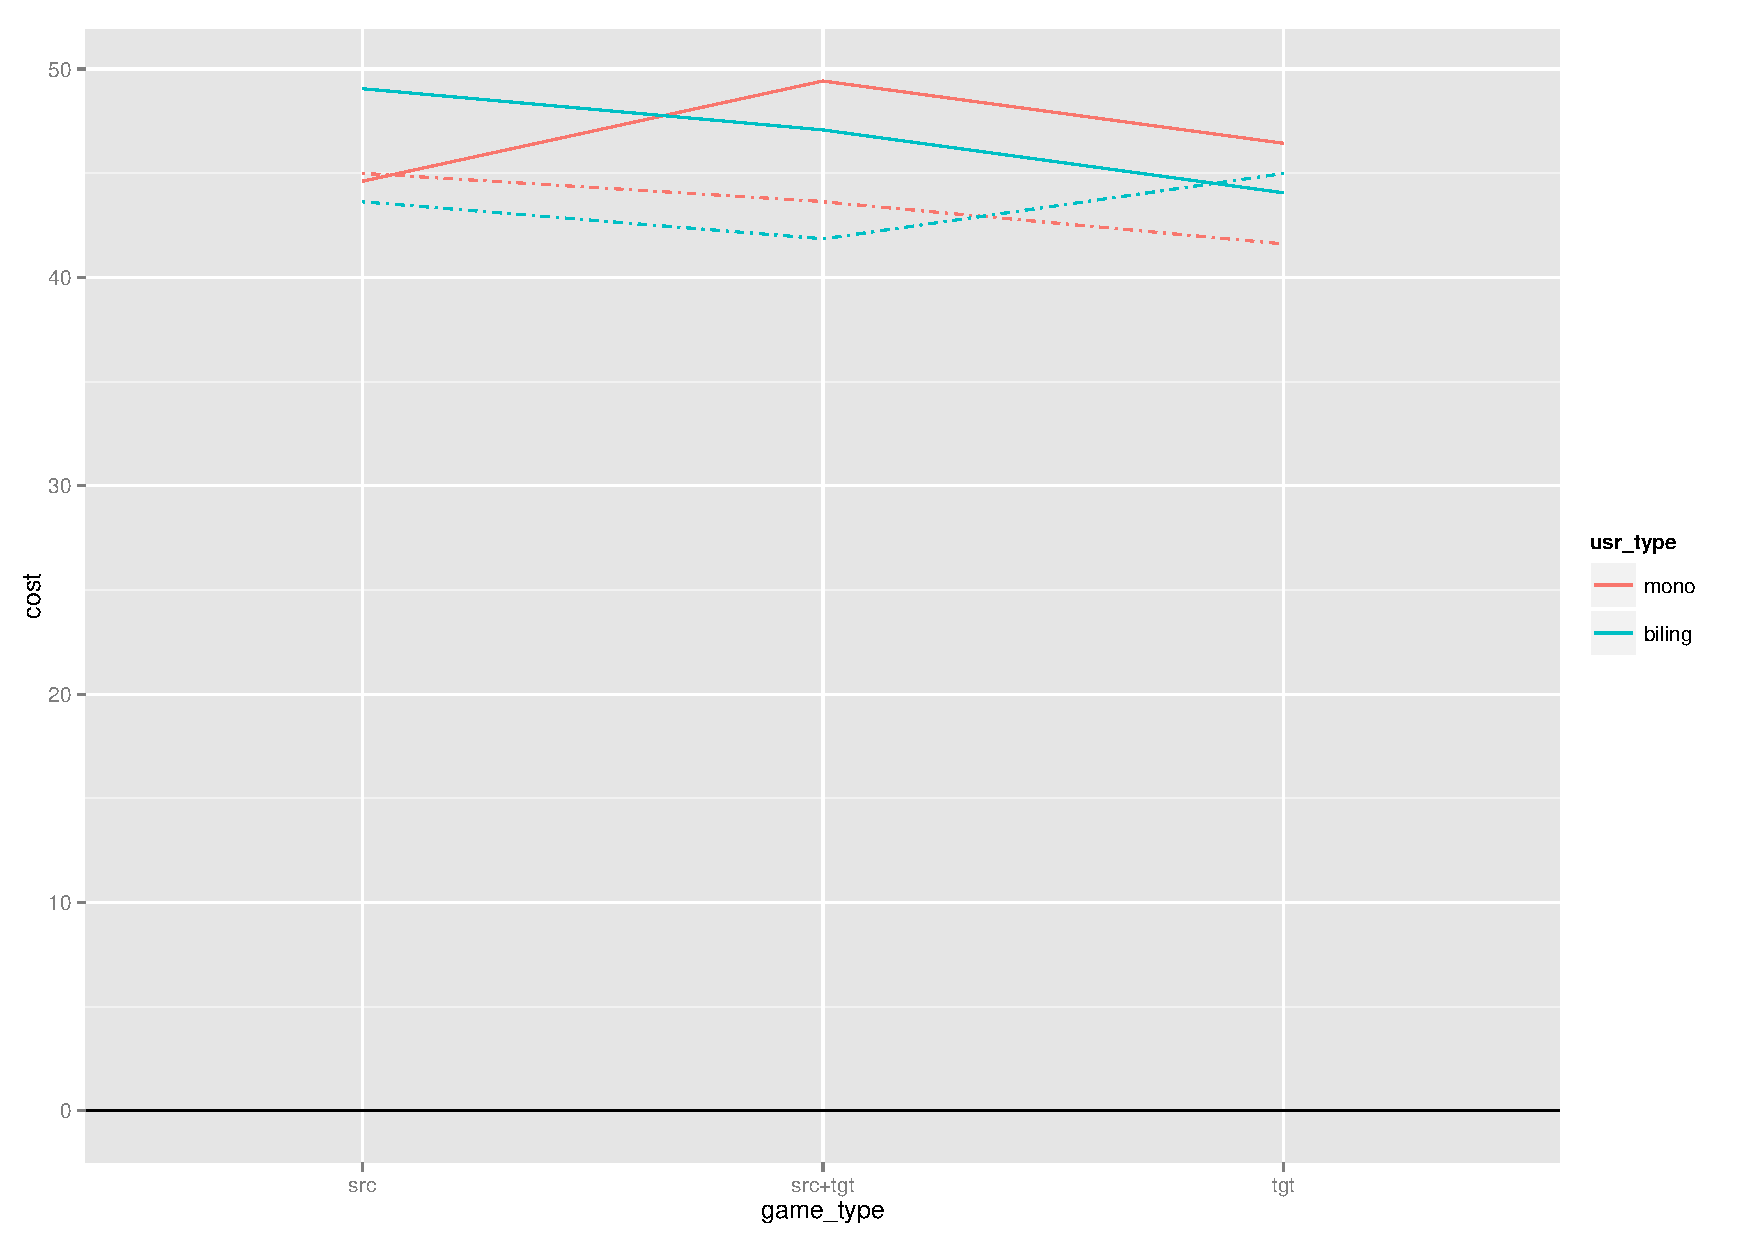
\includegraphics[scale=0.275]{data/cost_users_lm.pdf}
% \caption{Consistency of users vs humans and language model}
% \label{fig:costlm}
% \end{figure}
% \fi
\subsection{Is Bilingual Adequacy Necessary?}

Bilingual evaluators are considered to be the \emph{gold standard} for the evaluation of machine translation \cite{Dorr2011}. However, the use of monolingual evaluators has been previously advocated, since the end-users of MT are in fact monolingual \cite{Sanders2011}. The results obtained in this paper lead us to challenge the inclusion of \bil evaluators  for MT evaluation. %are really necessary for evaluating machine translation output. 
As seen in the results, \mono evaluators were slower than \bils, but they were more consistent in their evaluations. %Although in the \src \gamet they risked to evaluate only the readability of the translation (as also reported by some of our monolingual evaluators), there was no such risk in the remaining \gamets where the reference translation was provided. 
Given the open-ended nature of \bil evaluation (e.g. given a source text, they can formulate their  own set of plausible translations), we believe that the evaluations of \bils can be more subjective and prone to influence by the evaluator's background and knowledge of a specific subject.  Moreover,
 recruiting \bil evaluators can be harder and more expensive. %by the mismatch of their own mental translations with the MT output or the reference translation
We consider that consistency should be a primary goal of any evaluation task. Therefore, it seems more practical to rely only on \monos for the evaluation of machine translation. Our findings are in line with the observations in the post-editing community where \monos were more apt for the task and improved the fluency and comprehensibility of translations~\cite{mitchell2013community}. Our findings are also in partial agreement with White et al.~\shortcite{white1993evaluation} (which is not directly comparable to our work, as it does not compare monolinguals and bilinguals performing the same task), who state that less time is spent in evaluation techniques that use only target side information. 

%Our findings are in line with previous observations in the MT evaluation community where \monos seemed to perform better than \bils for a number of criteria (e.g. time) ~\cite{mitchell2013community,white1993evaluation}.

\subsection{Can Feedback Bias the Evaluation?}\label{ss:disc_feedback}
The process of evaluation can be cumbersome, especially if the evaluation sessions last for long; hence we used feedback to boost the engagement of participants throughout the evaluation process. This is a double-edged sword, as the feedback has the potential to bias the evaluators and influence their decision. %This is specially troublesome since we used scores coming from a different task (i.e. ranking) and from an automatic metric to compute feedback scores. 
\pagebreak

To rule-out any potential bias from the feedback, we investigated the effects that the progression in which the tasks were performed might have on the differences between the evaluator scores and the feedback scores. %standard deviation of the user's score with respect to the feedback scores 

If the evaluators \emph{learned} to reproduce the feedback scores, we would expect that the feedback error ($\tau_c$) would decrease as a function of time. \\
We calculated the feedback error as follows:

%Additionally, we measured the deviation with respect to the \emph{corrected} human raking scores used for \emph{feedback}, to get an idea of which type of users were \emph{closer} to the translation quality obtained with ranking. 
%We calculated the deviation $\tau$ as follows:

\begin{equation}
\tau_c^2 =   \frac{1}{N_c}\sum_{i \in T} \sum_{j\in C}(\tilde x_{ij} - f_i)^2
\end{equation}

\noindent where $f_i$ is the feedback score for translation $i$, and other variables are the same as in eq. ~\ref{eq:1}.

We fitted a linear model to the data, using the \gamet, the evaluator type and the progression (time) as predictors; and the feedback error as a response. We did not find that the progression had any significant effect ($p=0.2856$) on the feedback error.  This means that the feedback did not bias the scoring behavior of the evaluators.

\subsection{Can We do More with Eye-tracking?}
\Eye technology has proven useful in different scenarios related to translation.
%\paco{Here we give more examples of how it was used}
%So far, 
Yet, here we have only used the \eye device to measure the \emph{dwell} time an evaluator spends reading a specific portion of the screen. Nonetheless, one can think of more refined uses for this technology.

Potentially, using \eye can give us a fine-grained insight on how evaluators differentiate \emph{good} from \emph{bad} translations, making it easier to \emph{learn} the intrinsic rules of thumb that they use during the evaluation process. The applications for this are manifold. For example, by learning which type of errors (e.g. morphological, syntactic, semantic) can make a stronger impact on the reading behavior while evaluating, we could help to develop \emph{better} automatic MT evaluation metrics. Additionally, we can use gaze-data to model the evaluation score (or rank) given by an evaluator, and thus reduce the subjective score bias. This can help to alleviate the high variance found in evaluation. 

However, there are several challenges that need to be solved before moving forward in this nascent area. The most important is related to the accuracy of the \eye devices, which is a requirement to track which specific words are looked-at in the screen. 
\pagebreak

\Eye errors can be divided into two categories: variable (device-related precision) and systematic. Fortunately, the former has improved over the past years, and high-precision devices can be now acquired for only a few hundred dollars. The latter, however is more complex. Often, a loss in accuracy known as \emph{drift} is observed as time progresses, requiring frequent re-calibrations of the \eye device. \\
This can be due to evaluator movements, and other environmental factors. Reducing and eliminating drift is imperative to make progress in this area. Up to now, only heuristic approaches have been proposed \cite{mishra-carl-bhattacharyya:2012:ETNLP}, leaving plenty of room for improvement.


